\section{Results}
\label{SECIV}\label{sec:results}

We generated receiver operating characteristic (\textsc{roc}) curves for a selection of choices for the composite detection statistic threshold and the \textsc{svd} tolerance.  For each \textsc{roc} curve, or `run', we analyzed mock data with injections to assess detection efficiencies and mock data without injections to evaluate false alarm rates.

\subsection{Detector noise characteristics}

We tested the new detection method with mock Advanced \textsc{ligo} data having a power spectrum prescribed by the ``zero detuning, high power'' noise model in \cite{Shoemaker:2009p9770}.  Colored Gaussian noise is generated by passing 5 independent realizations of white Gaussian noise sampled at 16384 Hz through a bank of 5 third-order \textsc{iir} filters, then summing the filters' outputs.  This carefully designed filter bank reproduces the noise model very faithfully, but since it is composed of \textsc{iir} filters it can produce mock data in realtime very cheaply.  See \ref{appendix:mock-data} for implementation details. \editorial{In this section, we refer to aLIGO run parameters, but the results are actually using initial LIGO noise and initial LIGO parameters.  This will be fixed.}

\subsection{Injection population}

For each run, we performed about $10^4$ injections into our mock dataset.  Injections were 2PN post-Newtonian inspiral waveforms with component masses independently and identically distributed in $[1, 3]$ $M_\odot$.  Injections were tapered \editorial{Check --taper-injection option with Drew.} at a frequency of 10~Hz where they enter the Advanced \textsc{ligo} detection band.  This dictated that the longest injection waveform had a duration of 1~777~s.  In order to guarantee that no two injection waveforms overlapped in the data, the coalescence times of injections were spaced apart by {\color{red} 2~000~$\pm$~100~s}.  For the sake of economizing disk space, we simultaneously analyzed {\color{red} 16 statistically independent sets} of about $10^3$ injections apiece in the same {\color{red} 14 day} stretch of mock strain data.

Injections were distributed uniformly in log distance.  We used the following heuristic to provide a reasonably balanced number of distant, marginally detectable signals, and nearby, easily detected signals:
$$
d_\mathrm{min} = \frac{1}{2} \cdot \frac{\rho_\mathrm{candle}}{8.0 \cdot \min {d_\mathrm{eff}}}, \quad
d_\mathrm{max} = \frac{1}{4} \cdot \frac{\rho_\mathrm{candle}}{5.5 \cdot \max {d_\mathrm{eff}}}.
$$
Here, $\rho_\mathrm{candle}$ is a fiducially selected \textsc{snr}, and $d_\mathrm{eff}$ is the distance at which a face-on-system would produce a matched filter \textsc{snr} of $\rho_\mathrm{candle}$.

Orientations of injection sources are drawn uniformly, such that the sky location is distributed uniformly in $4\pi$ and the cosine of the binary inclination angle $\iota$ is distributed uniformly in $[0, \pi]$.

\subsection{Noninjection population}

We completed one injection-free pass over the 14~day dataset. \editorial{And **why**?  This part is too terse.}

\subsection{Triggering and data reduction}

For each template with parameters $\theta_i$, a trigger is recorded any time the absolute value of the \textsc{snr}, $|\rho(\theta_i)|$, is greater than a threshold $\rho^* = 5.5$, and is also a maximum over the 10~ms before and after. \editorial{This is a proposed trigger criterion that is much simpler than what we currently use.} A trigger is therefore an ordered triple $(t, i, \rho)$, recording the time, template number, and complex \textsc{snr} of an excursion in the outputs of the matched filter bank.

Offline, triggers for all templates collectively are clustered by time, such that within a sliding window of 4 seconds, all triggers except the one with the highest $\rho$ is kept.

For the injection-free passes, all clustered triggers are regarded as false alarms.  We accumulate the \textsc{snr}s of all of the false alarms into the set $\{|\rho|\}_\mathrm{false\,alarm}$.

For each injection, we check whether there was any clustered trigger that was within 2 seconds of the injection's time.  If there was, then the injection is considered to be recovered at the \textsc{snr} of that trigger.  Otherwise, the injection was not recovered because the \textsc{snr} threshold $\rho^*$ was not met, so we consider the injection to be recovered only at an \textsc{snr} of $\infty$.  From all found injections, we accumulate the injected distance and the recovered \textsc{snr} into the set $\{(d, |\rho|)\}_\mathrm{found}$.

\begin{figure}[htbp]
\begin{center}
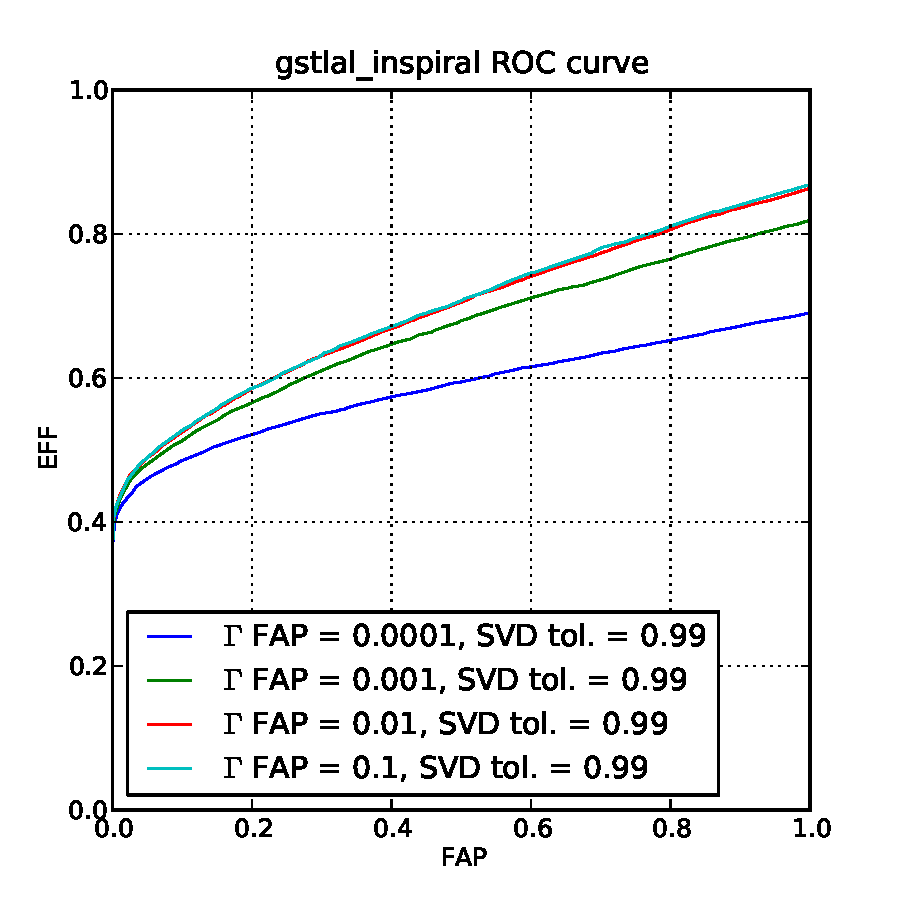
\includegraphics[scale=0.4]{figures/roc_99.pdf}
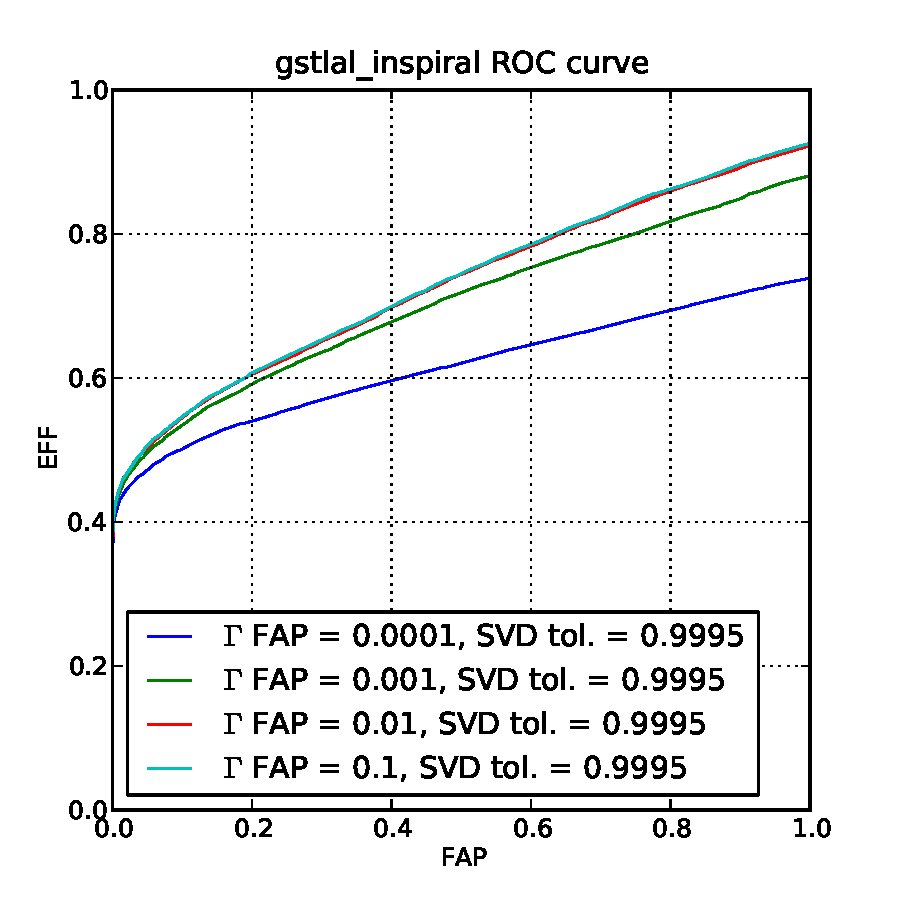
\includegraphics[scale=0.4]{figures/roc_9995.pdf}
\caption{Receiver operating characteristic (\textsc{roc}) curve of detection efficiency (\textsc{eff}) versus false alarm probability (\textsc{fap}).}
\label{fig:roc}
\end{center}
\end{figure}
